\documentclass{report}
\usepackage{tikz}
\usetikzlibrary{automata,positioning}

\begin{document}


% \begin{tikzpicture}
% % Draw the states
% \node[state]             (b) {blue-collar};
% \node[state, right  = of b] (w) {white-collar};
% \node[state, above  = of b] (e) {engineer};
% \node[state, right  = of e] (a) {artist};
% % Connect the states with arrows
% \draw[every loop]
%   (b) edge[bend right, auto=left]  node {0.6} (e)
%   (b) edge[bend right, auto=right] node {0.7} (a)
%   (w) edge[bend right, auto=left]  node {0.6} (e)
%   (w) edge[bend right, auto=left]  node {0.6} (a);
% \end{tikzpicture}

% % \begin{tikzpicture}
% % % Draw the states
% % \node[state]             (b) {blue-collar};
% % \node[state, right  = of b] (w) {white-collar};
% % \node[state, above  = of b] (e) {engineer};
% % \node[state, right  = of e] (a) {artist};
% % % Connect the states with arrows
% % % \draw[every loop]
% % % % (b) edge[bend right, auto=left]  node {0.6} (e)
% % % % (b) edge[bend right, auto=right] node {0.7} (a)
% % % % (s) edge[loop above]             node {0.4} (s)
% % % (r) edge[loop above]  
% % \end{tikzpicture}
Different starting conditions lead to different probabilities to transition to a variety of professions. Some people say that the probabilities depend on innate talent, there is probably some truth to the view that biology affects this probability but here I want to focus on the environmental aspect. Specifically, the idea of equality of opportunity.

First, let us begin by describing how things are. For the sake of simplicity assume there are only two possible professions, and that they mary each other such that there are only carpenter parents and mathematician parents. It should become clear soon enough that this generalizes for any number of starting positions and professions. In the image below, one should see that somebody born to carpenter(mathematician) parents has a $0.6\%(0.3\%)$ of becoming a carpenter and a $0.4\%(0.7\%)$ of becoming a mathematician. 

    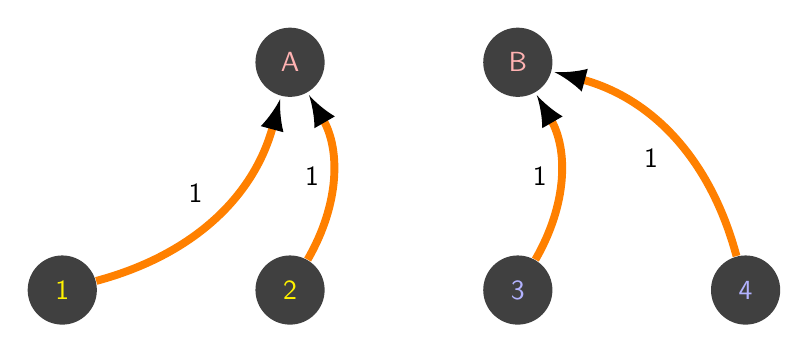
\begin{tikzpicture}[font=\sffamily]
    % Add the states
    \node[state,
          text=yellow,
          draw=none,
          fill=gray!50!black] (1) {1};
    \node[state,
          right=2cm of 1,
          text=yellow, 
          draw=none, 
          fill=gray!50!black] (2) {2};
   \node[state,
          right=2cm of 2,
          text=blue!30!white, 
          draw=none, 
          fill=gray!50!black] (3) {3};
   \node[state,
          right=2cm of 3,
          text=blue!30!white, 
          draw=none, 
          fill=gray!50!black] (4) {4};
   \node[state,
          above=2cm of 2,
          text=red!30!white, 
          draw=none, 
          fill=gray!50!black] (A) {A};
   \node[state,
          above=2cm of 3,
          text=red!30!white, 
          draw=none, 
          fill=gray!50!black] (B) {B};
    % Connect the states with arrows
\draw[every loop, 
	auto=right,
	line width = 1mm,
	>=latex,
	draw=orange]
	(1) edge[bend right, auto=left]  node {1} (A)
	(2) edge[bend right, auto=left]  node {1} (A)
	(3) edge[bend right, auto=left]  node {1} (B)
	(4) edge[bend right, auto=left]  node {1} (B);
   \end{tikzpicture}


    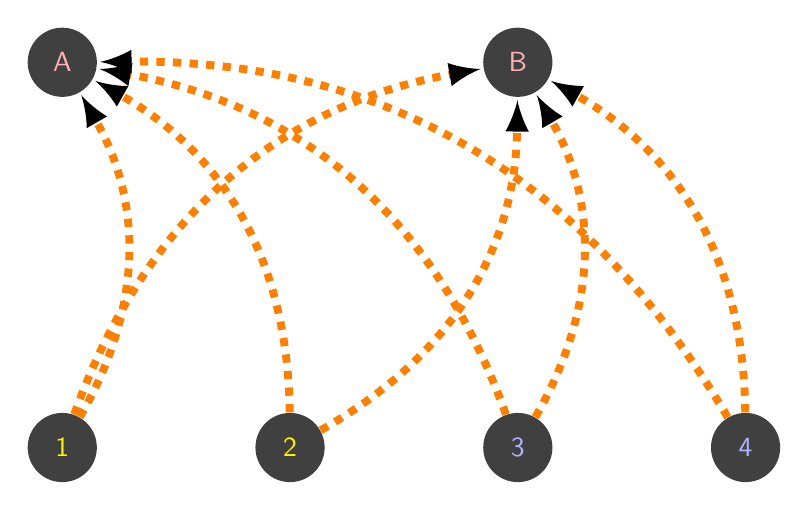
\begin{tikzpicture}[font=\sffamily]
    % Add the states
    \node[state,
          text=yellow,
          draw=none,
          fill=gray!50!black] (1) {1};
    \node[state,
          right=2cm of 1,
          text=yellow, 
          draw=none, 
          fill=gray!50!black] (2) {2};
   \node[state,
          right=2cm of 2,
          text=blue!30!white, 
          draw=none, 
          fill=gray!50!black] (3) {3};
   \node[state,
          right=2cm of 3,
          text=blue!30!white, 
          draw=none, 
          fill=gray!50!black] (4) {4};
   \node[state,
          above=4cm of 1,
          text=red!30!white, 
          draw=none, 
          fill=gray!50!black] (A) {A};
   \node[state,
          above=4cm of 3,
          text=red!30!white, 
          draw=none, 
          fill=gray!50!black] (B) {B};
    % Connect the states with arrows
\draw[every loop, dashed, 
	auto=right,
	line width = 1mm,
	>=latex,
	draw=orange]
	(1) edge[bend right, auto=left]  node {} (A)
	(2) edge[bend right, auto=left]  node {} (A)
	(1) edge[bend left, auto=left]  node {} (B)
	(2) edge[bend right, auto=left]  node {} (B)
	(3) edge[bend right, auto=left]  node {} (A)
	(4) edge[bend right, auto=left]  node {} (A)
	(3) edge[bend right, auto=left]  node {} (B)
	(4) edge[bend right, auto=left]  node {} (B);
   \end{tikzpicture}
  %  \draw[every loop,
      %    auto=right,
           % line width=1mm,
          %  >=latex,
         %   draw=orange,
        %    
       %   (b) edge[bend right, auto=left]  node {0.4} (e)
      %    (b) edge[bend left, auto=left]  node {0.6} (a)
     %     (w) edge[bend right, auto=right] node {0.7} (e)
    %      (w) edge[bend right, auto=right] node {0.3} (a);

Now under my interpretation of equality of opportunity, this picture shows a lack of equality of opportunity. For equality of opportunity to be achieved here, it must be that the transition probabilities from both states be equal. This seems like a fair representation of the concept. It should also be clear why this is terrible idea, it entails the abolition of the family. How can the parents fail to pass on even the slightest edge to their children about their own profession? Either the parents are neglecting their children to an absurd degree or the children have been confiscated from their parents. 

It should be clear that this is true even if children have different natural affinities, like below where I label children with math(carpenter) families that have math affinities as MMA(CMA), math(carpenter) families with carpenter affinities as MCA(CCA). Even if child which is naturally gifted in mathematics, will never have the same probability to transition to mathematics as a gifted child from a math family. As a rather technical note, it should be clear that if there is no equal total probability of transitioning to each profession, then some professions will gradually go extinct. 

    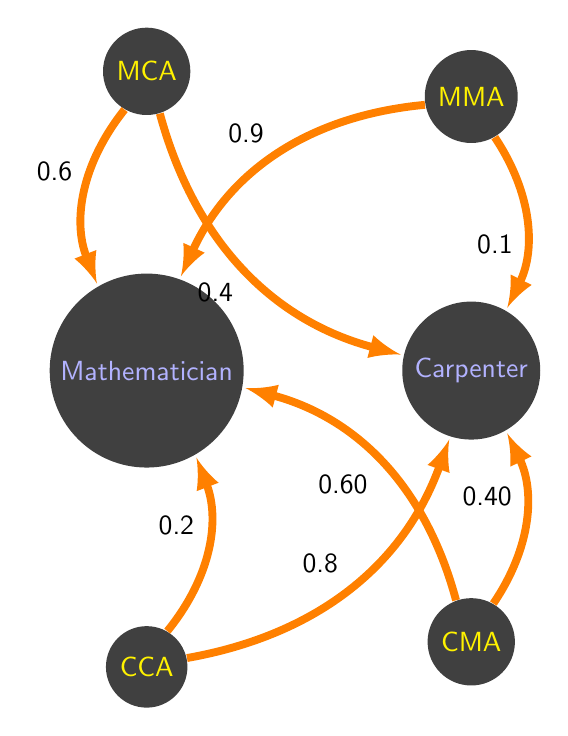
\begin{tikzpicture}[font=\sffamily]

   \node[state,
          text=blue!30!white, 
          draw=none, 
          fill=gray!50!black] (e) {Mathematician};
   \node[state,
          right=2cm of e,
          text=blue!30!white, 
          draw=none, 
          fill=gray!50!black] (a) {Carpenter};
    \node[state,
          below=2cm of a,
          text=yellow,
          draw=none,
          fill=gray!50!black] (b) {CMA};
    \node[state,
          below=2cm of e,
          text=yellow,
          draw=none,
          fill=gray!50!black] (cc) {CCA};
    \node[state,
          above=2cm of e,
          text=yellow, 
          draw=none, 
          fill=gray!50!black] (w) {MCA};
    \node[state,
          above=2cm of a,
          text=yellow, 
          draw=none, 
          fill=gray!50!black] (mm) {MMA};
    % Connect the states with arrows
    \draw[every loop,
          auto=right,
          line width=1mm,
          >=latex,
          draw=orange,
          fill=orange]
        (b) edge[bend right, auto=left]  node {0.60} (e)
        (b) edge[bend right, auto=left]  node {0.40} (a)
        (cc) edge[bend right, auto=left]  node {0.2} (e)
        (cc) edge[bend right, auto=left]  node {0.8} (a)
        (w) edge[bend right, auto=right] node {0.6} (e)
        (w) edge[bend right, auto=right] node {0.4} (a)
        (mm) edge[bend right, auto=right] node {0.9} (e)
        (mm) edge[bend left, auto=right] node {0.1} (a);
   \end{tikzpicture}

This is part of the sickness of trying to construct a rational order, most human constructs will have the property of stationarity. The rational construct has a tendency to destroy diversity under the guise of empathy. It should be clear that these rational constructions are an attack on the inheritance we have as humans, the family being the most vital. This is a problem with our intellect, it so happens that stationary constructs are simply easier to make. However, as our ideas become developed, we can better articulate principles that are in line with our inheritance. We just need to make sure that we supress the tendency to rationally construct until it is in line with our intuitions. 

In short, equality of opportunity ensures one of two things. Either a low diversity of opportunities, OR a lot of mediocrity. For everyone to have an equal probability of becoming everything, that must mean that either the professions in question are rather easy to learn OR it means everybody it means that nobody has learned enough to give them an advantage.

A better idea that equality of opportunity is ergodicity of wealth. The idea is rather simple, we want the wealth distribution to simply converge. 

    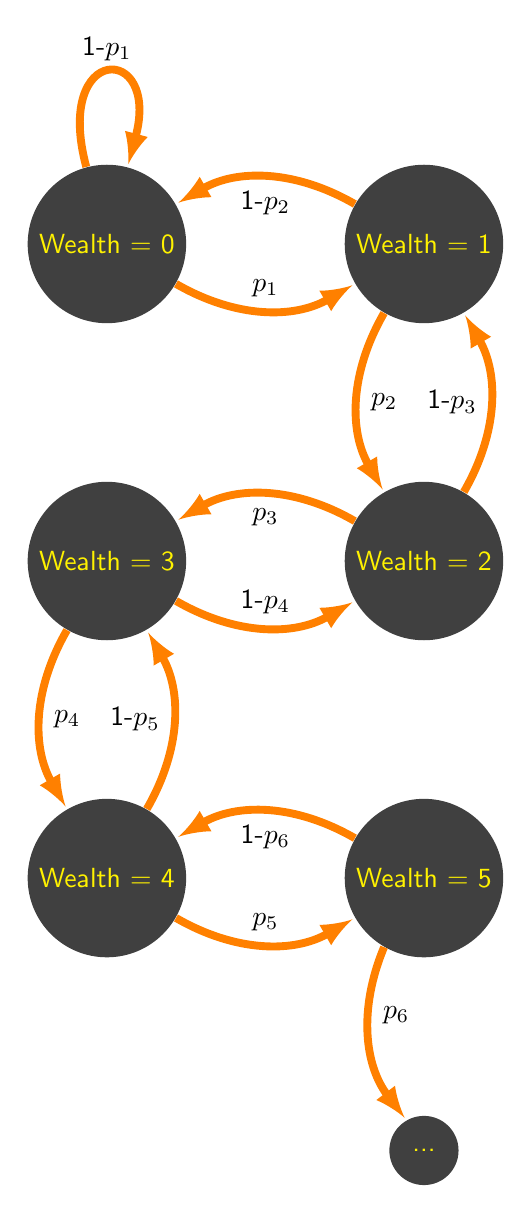
\begin{tikzpicture}[font=\sffamily]
   \node[state,
          text=yellow, 
          draw=none, 
          fill=gray!50!black] (0w) {Wealth = 0};
   \node[state,
          right=2cm of 0w,
          text=yellow, 
          draw=none, 
          fill=gray!50!black] (1w) {Wealth = 1};
    \node[state,
          below=2cm of 1w,
          text=yellow,
          draw=none,
          fill=gray!50!black] (2w) {Wealth = 2};
    \node[state,
          left=2cm of 2w,
          text=yellow,
          draw=none,
          fill=gray!50!black] (3w) {Wealth = 3};
    \node[state,
          below=2cm of 3w,
          text=yellow,
          draw=none,
          fill=gray!50!black] (4w) {Wealth = 4};
    \node[state,
          right=2cm of 4w,
          text=yellow,
          draw=none,
          fill=gray!50!black] (5w) {Wealth = 5};
    \node[state,
          below=2cm of 5w,
          text=yellow,
          draw=none,
          fill=gray!50!black] (etc) {...};
    Connect the states with arrows
    \draw[every loop,
          auto=right,
          line width=1mm,
          >=latex,
          draw=orange,
          fill=orange]
        (0w) edge[bend right, auto=left]  node {$p_1$} (1w)
        (0w) edge[loop above]  node {1-$p_1$} (0w)
        (1w) edge[bend right, auto=left]  node {$p_2$} (2w)
        (1w) edge[bend right, auto=left] node {1-$p_2$} (0w)
        (2w) edge[bend right, auto=left]  node {$p_3$} (3w)
        (2w) edge[bend right, auto=left]  node {1-$p_3$} (1w)
        (3w) edge[bend right, auto=left]  node {$p_4$} (4w)
        (3w) edge[bend right, auto=left]  node {1-$p_4$} (2w)
        (4w) edge[bend right, auto=left]  node {$p_5$} (5w)
        (4w) edge[bend right, auto=left]  node {1-$p_5$} (3w)
        (5w) edge[bend right, auto=left]  node {$p_6$} (etc)
        (5w) edge[bend right, auto=left]  node {1-$p_6$} (4w);
   \end{tikzpicture}

For simplicity we assume you can only jump up one bracket but the idea does not depend on a single jump. So we can now present what the criteria for ergodicity are: The probability of going higher has to be decreasing in wealth, so for example$p_2>p_1$ and $p_3>p_2$. Technically, ergodicity in this context just means that the distribution of wealth can be modelled. That is, if the rich get richer faster than the poor, then the distribution kind of explodes(loses continuity). It is not clear WHY we should care about whether the academic should be able to model the distribution as a normative criteria, but at the very least this criterion allows for more diversity than a concept like equality of opportunity and perhaps more importantly, it does not call for abolition of the family. 

The most obvious problem here is the measure, wealth, it is not clear what it refers to, indeed this is the kind of urbanite assumption that gets baked in that misses everything that you cannot buy. If wealth measures physical stuff, then clearly this either entails a zero sum world OR that humans can infinitely expand their physical consumption. Yet it should be clear that if Anna wants halloumi but prefers blue cheese, and Bob has blue cheese but prefers halloumi. Clearly if they exchanged, the total amount of physical wealth would stay constant but there would be more value. 

So we could interpret wealth as a non-physical category. But then, we might have that somebody is better off by having lower wealth! Which means the criteria loses it's normative force. Anyway, though, I don't think this ergodic criterion is all that great, it is still heuristically better than equality of opportunity. 

note: I am using the word ergodicity rather loosely here but I think it conveys the point. 

\end{document}